\section{Casi d'uso}
\subsection{Scopo}
Lo scopo di questa sezione è la descrizione in elenco di tutti i casi d'uso individuati dal gruppo, in riferimento alle funzionalità dell'applicazione.
\subsection{Attori}
Come accordato con il proponente, non essendo richiesto alcun servizio di autenticazione attraverso un login o una registrazione, è presente un solo attore che può interagire con l'applicazione web:

\begin{figure}[h]

\includegraphics[width=1cm]{section/Images/Utente.png}
\centering
\caption{Gerarchia attori}
\end{figure}

\begin{description}
\item[Utente]:
Si riferisce all'utente utilizzatore che può accedere alla piattaforma.
\end{description}
Per un eventuale gestione di dati in più sessioni è quindi richiesta la funzionalità di poter salvare il proprio lavoro in un file scaricabile, che può poi essere successivamente caricato sulla piattaforma permettendo la ripresa del lavoro.
\subsection{Elenco casi d'uso}
Di seguito sono riportati tutti i casi d'uso che coinvolgono l'utente:
\begin{figure}[h]
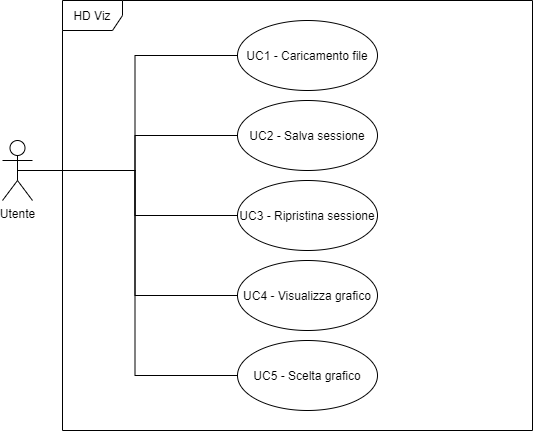
\includegraphics[width=\linewidth]{section/Images/HDviz.png}
\centering
\caption{Casi d'uso dell'utente}
\end{figure}
\subsubsection{UC1 - Caricamento del dataset}
\begin{figure}[h]
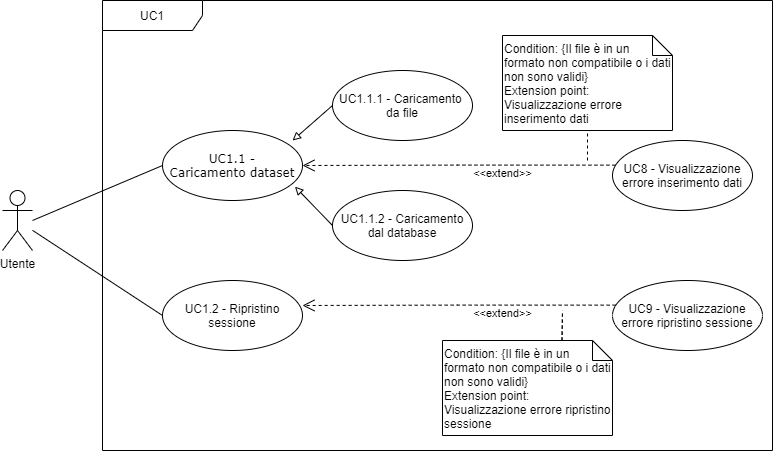
\includegraphics[width=\linewidth]{section/Images/UC1.png}
\centering
\caption{UC1 - Caricamento del dataset}
\end{figure}
\begin{itemize}
	\item \textbf{Attore primario}: Utente.
	\item \textbf{Precondizioni}: Il sistema è raggiungibile e funzionante.
	\item \textbf{Postcondizioni}: Viene visualizzato un messaggio che avvisa l'utente del corretto caricamento dei dati e della loro validità.
	\item \textbf{Scenario principale}:
		\begin{enumerate}
			\item L'utente accede al sistema;
			\item L'utente sceglie come ricavare i dati:
				\begin{enumerate}[(a)]
			\item L'utente seleziona la funzionalità "carica file" [UC1.1];
			\item L'utente seleziona un dataset tra quelli disponibili nel database [UC1.2].
				\end{enumerate}
		\end{enumerate}
	\item \textbf{Estensioni}:
	\begin{enumerate}[(a)]
		\item Nel caso in cui il file sia in un formato sbagliato o i dati non sono validi:
		\begin{enumerate}[1.]
			\item i dati non vengono caricati nel sistema;
			\item viene visualizzato un errore esplicativo [UC7].
		\end{enumerate}
	\end{enumerate}
\end{itemize}

\subsubsection{UC1.1 - Caricamento dataset da file}

\begin{itemize}
	\item \textbf{Attore primario}: Utente.
	\item \textbf{Precondizioni}: Il sistema è raggiungibile e funzionante. L'utente ha a disposizione un dataset in formato CSV.
	\item \textbf{Postcondizioni}: I dati presenti nel file vengono caricati nel sistema. Viene visualizzato un messaggio che avvisa l'utente del corretto caricamento e della validità dei dati.
	\item \textbf{Scenario principale}: L'utente sceglie di caricare un dataset personale o ricavato da altre fonti esterne.
	
\end{itemize}

\subsubsection{UC1.2 - Caricamento dataset dal database}

\begin{itemize}
	\item \textbf{Attore primario}: Utente.
	\item \textbf{Precondizioni}: Il sistema è raggiungibile e funzionante. L'utente effettua una query dal database disponibile per prelevare il dataset.
	\item \textbf{Postcondizioni}: I dati vengono caricati nel sistema. Viene visualizzato un messaggio che avvisa l'utente del corretto caricamento e della loro validità.
	\item \textbf{Scenario principale}: L'utente sceglie di caricare un dataset tra quelli presenti nel database.
	
\end{itemize}


  
\subsection{UC2 - Selezione delle dimensioni da utilizzare}
\begin{itemize}
	\item \textbf{Attore primario}: Utente;
	\item \textbf{Precondizioni}: L'utente ha caricato i dati nel sistema [UC1];
	\item \textbf{Postcondizioni}: Le dimensioni scelte vengono aggiornate nel sistema e i dati sono pronti per essere visualizzati [UC6];
	\item \textbf{Scenario principale}:
		\begin{enumerate}
			\item All'utente viene presentata una schermata con tutte le dimensioni presenti nel dataset caricato già selezionate di default;
			\item Per ogni dimensione è presente una cella da selezionare nel caso la si voglia utilizzare o meno;
			\item L'utente seleziona le dimensioni che desidera analizzare.
		\end{enumerate}
	\item \textbf{Estensioni:}
		\begin{enumerate}[(a)]
			\item Nel caso in cui l'utente non abbia selezionato nessuna dimensione:
			\begin{enumerate}[1.]
				\item Le dimensioni non vengono aggiornate nel sistema;
				\item Viene visualizzato un messaggio d'errore esplicativo [UC12].
			\end{enumerate}
		\end{enumerate}
\end{itemize}
\newpage
\subsubsection{UC3 - Scelta della \glo{visualizzazione}}
\begin{figure}[h]
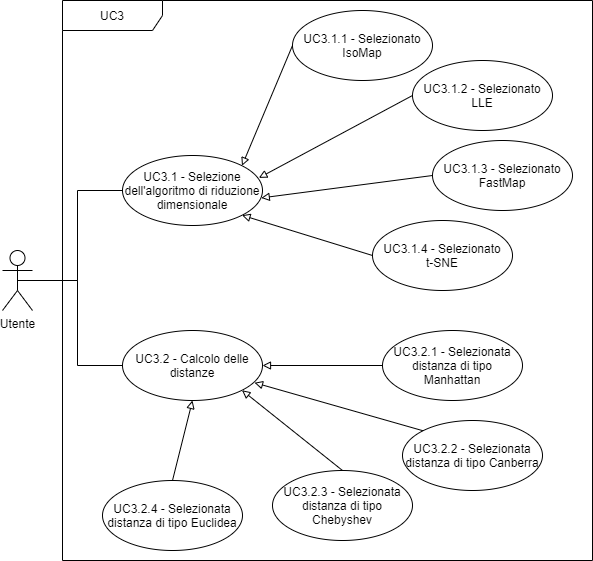
\includegraphics[width=\linewidth]{section/Images/UC3.png}
\centering
\caption{UC3 - Scelta della visualizzazione}
\end{figure}
\begin{itemize}
	\item \textbf{Attore primario}: Utente.
	\item \textbf{Precondizioni}: L'utente ha caricato dei dati nel sistema [UC1] e ha selezionato le dimensioni da utilizzare [UC2].
	\item \textbf{Postcondizioni}: Viene mostrata la visualizzazione scelta, con possibilità di personalizzazione [UC4].
	\item \textbf{Scenario principale}: L'utente seleziona una visualizzazione tra quelle disponibili.
	\item \textbf{Generalizzazioni}: L'utente seleziona una delle seguenti opzioni disponibili:
		\begin{enumerate}[(a)]
			\item \glo{\textit{Scatter Plot Matrix}} [UC3.1]
			\item \glo{\textit{Heat Map}} [UC3.2]
			\item \glo{\textit{Force Field}} [UC3.3]
			\item \glo{\textit{Proiezione Lineare Multi Asse}} [UC3.4]
		\end{enumerate}
	\item \textbf{Estensioni}:
	\begin{enumerate}[(a)]
		\item Nel caso in cui non è stato caricato alcun dato o non è stata scelta alcuna dimensione:
		\begin{enumerate}[1.]
			\item Il grafico non viene visualizzato;
			\item Viene visualizzato un errore esplicativo [UC9].
		\end{enumerate}
	\end{enumerate}
\end{itemize}
\subsection{UC4 - Modifica della riduzione dimensionale tramite algoritmo}
\begin{figure}[h]
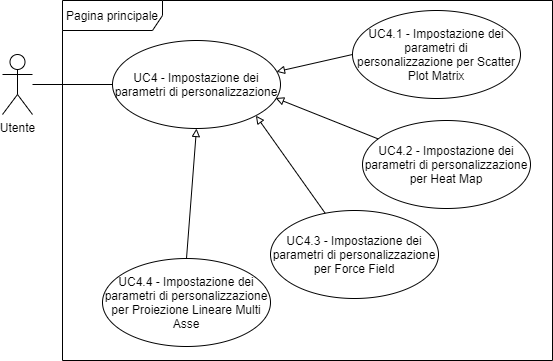
\includegraphics[width=9cm]{Section/Images/UC4.png}
\centering
\caption{UC4 - Modifica della riduzione dimensionale tramite algoritmo}
\end{figure}
\begin{itemize}
	\item \textbf{Attore primario}: Utente;
	\item \textbf{Precondizioni}: L'utente ha scelto l'algoritmo di riduzione dimensionale [UC3.1];
	\item \textbf{Postcondizioni}: I parametri di personalizzazione dell'algoritmo sono stasi impostati e vengono create il numero di dimensioni scelte, pronte per essere visualizzare [UC5];
	\item \textbf{Scenario principale}: L'utente
	
	\begin{enumerate}
		\item Seleziona il numero di dimensioni da ricavare dalla riduzione dimensionale [UC4.1];
		\item Personalizza i parametri dell'algoritmo di riduzione dimensionale selezionato secondo le sue esigenze [UC4.2].
	\end{enumerate}		
\end{itemize}

\subsubsection{UC4.1 - Selezione del numero di dimensioni}

\begin{itemize}
	\item \textbf{Attore primario}: Utente;
	
	\item \textbf{Precondizioni}: L'utente ha scelto un algoritmo di riduzione dimensionale [UC3.1];
	
	\item \textbf{Postcondizioni}: L'utente ha selezionato il numero di dimensioni che vuole ottenere dal processo di riduzione dimensionale;
	
	\item \textbf{Scenario principale}: L'utente decide il numero di dimensioni da ricavare selezionando un numero tra l'intervallo disponibile.
\end{itemize}	
	
\newpage	
	
\subsubsection{UC4.2 - Impostazione dei parametri dell'algoritmo}
\begin{figure}[h]
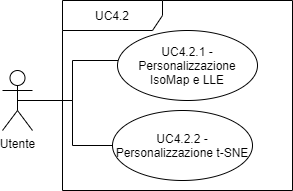
\includegraphics[width=9cm]{Section/Images/UC4.2.png}
\centering
\caption{UC4.2 - Impostazione dei parametri dell'algoritmo}
\end{figure}
\begin{itemize}
	\item \textbf{Attore primario}: Utente;
	
	\item \textbf{Precondizioni}: L'utente ha scelto un algoritmo di riduzione dimensionale [UC3.1];
	
	\item \textbf{Postcondizioni}: L'utente ha impostato i parametri personalizzabili dell'algoritmo;
	
	\item \textbf{Scenario principale}: L'utente imposta i parametri specifici dell'algoritmo selezionato.
	
		\item \textbf{Generalizzazioni}: L'utente imposta i parametri di personalizzazione dell'algoritmo scelto:
	\begin{enumerate}[(a)]
		\item Personalizzazione \glo{\textit{IsoMap}} e \glo{\textit{LLE}} [UC4.2.1];
		\item Personalizzazione \glo{\textit{t-SNE}} [UC4.2.2];
	\end{enumerate}
\end{itemize}		
		

\subsubsection{UC4.2.1 - Personalizzazione IsoMap e LLE}
\begin{itemize}
	\item \textbf{Attore primario}: Utente;
	
	\item \textbf{Precondizioni}: L'utente ha scelto l'algoritmo \textit{IsoMap} [UC3.1.1] oppure \textit{LLE} [UC3.1.2];
	
	\item \textbf{Postcondizioni}: L'algoritmo viene impostato con le personalizzazioni dell'utente;
	
	\item \textbf{Scenario principale}: L'utente seleziona il numero di punti vicini (\glo{\textit{neighbors}}), tra l'intervallo disponibile, per la stima approssimativa del \glo{\textit{manifold}}.

\end{itemize}

\newpage

\subsubsection{UC4.2.2 - Personalizzazione t-SNE}
\begin{figure}[h]
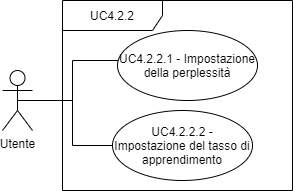
\includegraphics[width=9cm]{Section/Images/UC4.2.2.png}
\centering
\caption{UC4.2.2 - Personalizzazione t-SNE}
\end{figure}
\begin{itemize}
	\item \textbf{Attore primario}: Utente;
	
	\item \textbf{Precondizioni}: L'utente ha scelto l'algoritmo \textit{t-SNE} [UC3.1.4];
	
	\item \textbf{Postcondizioni}: L'algoritmo viene impostato con le personalizzazioni dell'utente;
	
	\item \textbf{Scenario principale}: L'utente decide:

\begin{enumerate}
\item Impostazione della perplessità [UC4.2.2.1];
\item Impostazione del tasso di apprendimento (\glo{\textit{Epsilon}}) [UC4.2.2.2];
\end{enumerate}	

\end{itemize}
	
	
\paragraph{UC4.2.2.1 - Impostazione della perplessità}
\begin{itemize}
	\item \textbf{Attore primario}: Utente;
	
	\item \textbf{Precondizioni}: L'utente ha scelto l'algoritmo \textit{t-SNE} [UC3.1.4];
	
	\item \textbf{Postcondizioni}: L'algoritmo viene impostato con le personalizzazioni dell'utente;
	
	\item \textbf{Scenario principale}: L'utente imposta il valore, tra l'intervallo disponibile, per bilanciare gli aspetti globali e locali dei dati.

\end{itemize}
	
\paragraph{UC4.2.2.2 - Impostazione del tasso di apprendimento}
\begin{itemize}
	\item \textbf{Attore primario}: Utente;
	
	\item \textbf{Precondizioni}: L'utente ha scelto l'algoritmo \textit{t-SNE} [UC3.1.4];
	
	\item \textbf{Postcondizioni}: L'algoritmo viene impostato con le personalizzazioni dell'utente;
	
	\item \textbf{Scenario principale}: L'utente imposta il valore, tra l'intervallo disponibile, del tasso di apprendimento dell'algoritmo.

\end{itemize}

\subsubsection{UC4.3 - Assegnazione del nome alle dimensioni create}

\begin{itemize}
	\item \textbf{Attore primario}: Utente;
	
	\item \textbf{Precondizioni}: L'utente ha scelto un algoritmo di riduzione dimensionale [UC3.1];
	
	\item \textbf{Postcondizioni}: L'utente ha assegnato i nomi alle dimensioni che andrà a creare;
	
	\item \textbf{Scenario principale}: L'utente assegna il nome alle dimensioni che sta creando nell'apposito campo d'input; il nome scelto sarà seguito da un numero crescente, che dipende dal numero di dimensioni generate. Se non modificato vengono mantenuti i nomi di default, costituiti dal nome dell'algoritmo scelto.

\end{itemize}	

\subsection{UC5 - Scelta della \glo{visualizzazione}}
\begin{figure}[h]
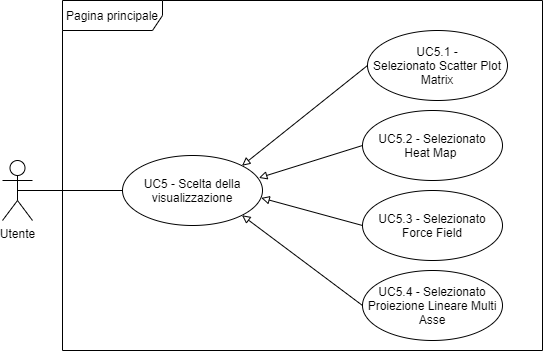
\includegraphics[width=\linewidth]{Section/Images/UC5.png}
\centering
\caption{UC5 - Scelta della visualizzazione}
\end{figure}
\begin{itemize}
	\item \textbf{Attore primario}: Utente;
	\item \textbf{Precondizioni}: L'utente ha caricato dei dati nel sistema e ha selezionato le dimensioni da utilizzare [UC2].
	\item \textbf{Postcondizioni}: Viene mostrata la visualizzazione scelta, con possibilità di personalizzazione [UC6]. La scelta viene salvata nel sistema.
	\item \textbf{Scenario principale}: L'utente seleziona la visualizzazione che vuole utilizzare tra quelle disponibili.
	\item \textbf{Generalizzazioni}: L'utente seleziona una delle seguenti opzioni:
		\begin{enumerate}
			\item \glo{\textit{Scatter Plot Matrix}} [UC5.1];
			\item \glo{\textit{Heat Map}} [UC5.2];
			\item \glo{\textit{Force Field}} [UC5.3];
			\item \glo{\textit{Proiezione Lineare Multi Asse}} [UC5.4].
		\end{enumerate}

\end{itemize}